\section{Held-out results (Level 1)}
\label{sec:results}

Table~\ref{tab:heldout} and Figure~\ref{fig:heldout} give the held-out success of every
family; Table~\ref{tab:differences} gives every declared difference, and
Figure~\ref{fig:differences} plots the comparisons that bear on H2, H2-c and H3. Each family
ran \rf{l1.lift.n} held-out starts per training seed on each task, once, after the Level~1
freeze (commit \texttt{\rf{l1.git}}).

\begin{table}[t]
\centering\small
\caption{Held-out success (\%) per family: successes over episodes, the mean over the three
training seeds with the hierarchical bootstrap's \rf{proto.level}\,\% interval, and the per-seed rates.}
\label{tab:heldout}
\resizebox{\linewidth}{!}{% Generated by scripts/paper_assets.py (DECISIONS D-094). Do not edit.
% Sources (path sha256):
%   reports/session7/results/results.json b8b097c38765c588711615917e3cfd5be6847e63083ddebe92f0f1488672408c
\begin{tabular}{lrrrrrr}
\toprule
Family & Lift $k/n$ & Lift success \% & Lift per seed & Can $k/n$ & Can success \% & Can per seed \\
\midrule
BC-MLP & 136/150 & 90.7 [83.3, 96.7] & 88, 92, 92 & 115/150 & 76.7 [62.7, 90.0] & 68, 88, 74 \\
BC-RNN & 150/150 & 100.0 [100.0, 100.0] & 100, 100, 100 & 144/150 & 96.0 [89.3, 100.0] & 92, 100, 96 \\
BC-MLP-chunk & 147/150 & 98.0 [94.0, 100.0] & 98, 100, 96 & 144/150 & 96.0 [88.7, 100.0] & 96, 92, 100 \\
Diffusion U-Net & 146/150 & 97.3 [93.3, 100.0] & 98, 96, 98 & 143/150 & 95.3 [89.3, 100.0] & 92, 98, 96 \\
Random (uniform) & 0/50 & 0.0 [0.0, 0.0] & 0 & 0/50 & 0.0 [0.0, 0.0] & 0 \\
\bottomrule
\end{tabular}
}
\end{table}

\begin{figure}[t]
\centering
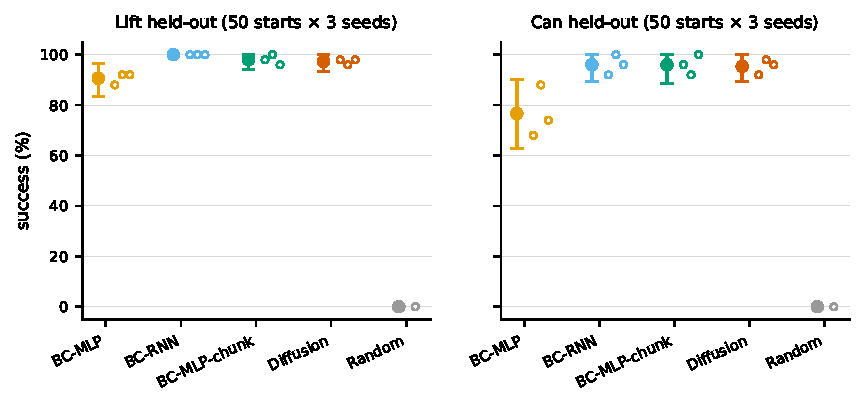
\includegraphics[width=\linewidth]{generated/figures/heldout_success.pdf}
\caption{Held-out success per family and task. Filled markers: mean over seeds with the
bootstrap \rf{proto.level}\,\% interval; open markers: the three training seeds.}
\label{fig:heldout}
\end{figure}

\paragraph{H1.} Every trained family separates from the random-action baseline, which never
succeeds, on both tasks (Table~\ref{tab:differences}).

\paragraph{Lift.} Lift is close to saturated: BC-RNN succeeds on every held-out start
(\rf{l1.lift.bcrnn.succ}\,\%), BC-MLP-chunk on \rf{l1.lift.chunk.succ}\,\% and diffusion on
\rf{l1.lift.diff.succ}\,\%. The only separated learned comparison is H3: BC-RNN exceeds BC-MLP
by \rf{l1.lift.bcrnn-bcmlp.d}\,pp [\rf{l1.lift.bcrnn-bcmlp.lo}, \rf{l1.lift.bcrnn-bcmlp.hi}].
Diffusion's advantage over BC-MLP (\rf{l1.lift.diff-bcmlp.d}\,pp
[\rf{l1.lift.diff-bcmlp.lo}, \rf{l1.lift.diff-bcmlp.hi}]) is not separated, although the
declared secondary outcome, censored episode length, is (\rf{l1.lift.len.diff-bcmlp.d} steps
[\rf{l1.lift.len.diff-bcmlp.lo}, \rf{l1.lift.len.diff-bcmlp.hi}], mostly from success), nor is its
difference from BC-RNN (\rf{l1.lift.diff-bcrnn.d}\,pp) or from BC-MLP-chunk
(\rf{l1.lift.diff-chunk.d}\,pp).

\paragraph{Can.} On Can, BC-MLP is the clear outlier (\rf{l1.can.bcmlp.succ}\,\%), while the
other three families lie within one point of each other (\rf{l1.can.bcrnn.succ},
\rf{l1.can.chunk.succ} and \rf{l1.can.diff.succ}\,\%). The primary H2 comparison is separated:
diffusion exceeds BC-MLP by \rf{l1.can.diff-bcmlp.d}\,pp [\rf{l1.can.diff-bcmlp.lo},
\rf{l1.can.diff-bcmlp.hi}]. The H2-c control does not support attributing that advantage to
the generative model: diffusion minus BC-MLP-chunk is \rf{l1.can.diff-chunk.d}\,pp
[\rf{l1.can.diff-chunk.lo}, \rf{l1.can.diff-chunk.hi}], is not separated (which is not evidence of equality). BC-RNN
also separates from BC-MLP (H3: \rf{l1.can.bcrnn-bcmlp.d}\,pp [\rf{l1.can.bcrnn-bcmlp.lo},
\rf{l1.can.bcrnn-bcmlp.hi}]), although it differs from BC-MLP in its architecture as well as in
its history. With privileged state on these two tasks, these data therefore give no evidence
that the generative head adds to observation history and chunking. That BC-MLP-chunk
(\rf{l1.can.chunk.succ}\,\%) also exceeds BC-MLP (\rf{l1.can.bcmlp.succ}\,\%) is visible in
Table~\ref{tab:heldout}, but it is not a declared comparison and is exploratory. A further difference between the heads, the diffusion sampler's bound on
its actions, is discussed in Section~\ref{sec:limitations}.

\begin{table}[t]
\centering\small
\caption{Declared held-out differences $A - B$ with the hierarchical paired bootstrap's
\rf{proto.level}\,\% interval. Success in percentage points; censored episode length in control steps,
with failures counted at the horizon (negative is faster). Intervals are not adjusted for
the \rf{proto.ncomparisons} success comparisons per task.}
\label{tab:differences}
\resizebox{\linewidth}{!}{% Generated by scripts/paper_assets.py (DECISIONS D-094). Do not edit.
% Sources (path sha256):
%   docs/FINAL_TEST_FREEZE.md 6a3c6874c4bc1857efe46ccb05c0a1fa68247671fc9a96f5f54ce079aa9153e9
%   reports/session7/results/results.json b8b097c38765c588711615917e3cfd5be6847e63083ddebe92f0f1488672408c
\begin{tabular}{llll}
\toprule
 & Difference $A - B$ & Lift & Can \\
\midrule
\multicolumn{4}{l}{\emph{Success (percentage points)}} \\
H1 & BC-MLP $-$ Random (uniform) & \ensuremath{+}90.7 [\ensuremath{+}83.3, \ensuremath{+}96.7], separated (\ensuremath{+}) & \ensuremath{+}76.7 [\ensuremath{+}62.7, \ensuremath{+}90.0], separated (\ensuremath{+}) \\
H1 & BC-RNN $-$ Random (uniform) & \ensuremath{+}100.0 [\ensuremath{+}100.0, \ensuremath{+}100.0], separated (\ensuremath{+}) & \ensuremath{+}96.0 [\ensuremath{+}89.3, \ensuremath{+}100.0], separated (\ensuremath{+}) \\
H1 & BC-MLP-chunk $-$ Random (uniform) & \ensuremath{+}98.0 [\ensuremath{+}94.0, \ensuremath{+}100.0], separated (\ensuremath{+}) & \ensuremath{+}96.0 [\ensuremath{+}88.7, \ensuremath{+}100.0], separated (\ensuremath{+}) \\
H1 & Diffusion U-Net $-$ Random (uniform) & \ensuremath{+}97.3 [\ensuremath{+}93.3, \ensuremath{+}100.0], separated (\ensuremath{+}) & \ensuremath{+}95.3 [\ensuremath{+}89.3, \ensuremath{+}100.0], separated (\ensuremath{+}) \\
H2 & Diffusion U-Net $-$ BC-MLP & \ensuremath{+}6.7 [\ensuremath{-}0.7, \ensuremath{+}14.7], not separated & \ensuremath{+}18.7 [\ensuremath{+}4.7, \ensuremath{+}32.7], separated (\ensuremath{+}) \\
H2 & Diffusion U-Net $-$ BC-RNN & \ensuremath{-}2.7 [\ensuremath{-}6.7, \ensuremath{+}0.0], not separated & \ensuremath{-}0.7 [\ensuremath{-}8.0, \ensuremath{+}6.7], not separated \\
H2-c & Diffusion U-Net $-$ BC-MLP-chunk & \ensuremath{-}0.7 [\ensuremath{-}5.3, \ensuremath{+}4.7], not separated & \ensuremath{-}0.7 [\ensuremath{-}8.7, \ensuremath{+}7.3], not separated \\
H3 & BC-RNN $-$ BC-MLP & \ensuremath{+}9.3 [\ensuremath{+}3.3, \ensuremath{+}16.7], separated (\ensuremath{+}) & \ensuremath{+}19.3 [\ensuremath{+}5.3, \ensuremath{+}34.0], separated (\ensuremath{+}) \\
\midrule
\multicolumn{4}{l}{\emph{Censored episode length (steps; failures count 400)}} \\
H2 & Diffusion U-Net $-$ BC-MLP & \ensuremath{-}28.9 [\ensuremath{-}59.4, \ensuremath{-}1.6], separated (\ensuremath{-}) & \ensuremath{-}56.0 [\ensuremath{-}98.0, \ensuremath{-}14.7], separated (\ensuremath{-}) \\
H2 & Diffusion U-Net $-$ BC-RNN & \ensuremath{+}11.0 [\ensuremath{+}1.1, \ensuremath{+}25.1], separated (\ensuremath{+}) & \ensuremath{+}2.1 [\ensuremath{-}18.5, \ensuremath{+}22.7], not separated \\
H2-c & Diffusion U-Net $-$ BC-MLP-chunk & \ensuremath{+}2.8 [\ensuremath{-}15.6, \ensuremath{+}20.0], not separated & \ensuremath{+}9.5 [\ensuremath{-}13.0, \ensuremath{+}33.3], not separated \\
H3 & BC-RNN $-$ BC-MLP & \ensuremath{-}39.9 [\ensuremath{-}67.8, \ensuremath{-}16.2], separated (\ensuremath{-}) & \ensuremath{-}58.1 [\ensuremath{-}100.3, \ensuremath{-}16.7], separated (\ensuremath{-}) \\
\bottomrule
\end{tabular}
}
\end{table}

\begin{figure}[t]
\centering
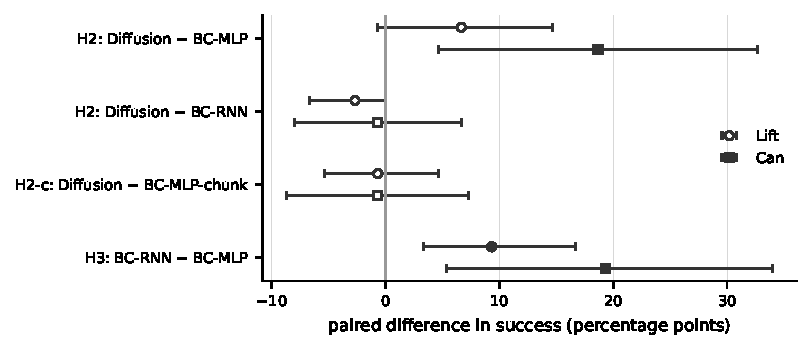
\includegraphics[width=\linewidth]{generated/figures/differences.pdf}
\caption{The H2, H2-c and H3 differences in held-out success with their \rf{proto.level}\,\% intervals.
Filled markers are separated (the interval excludes zero).}
\label{fig:differences}
\end{figure}

\paragraph{How much the verdicts depend on the interval method.} The seed-level sensitivity
analysis (Section~\ref{sec:protocol}; Table~\ref{tab:sens-main}; not preregistered) changes
\rf{sens.l1.changed} of the \rf{sens.l1.n} Level~1 verdicts. Both separated Can comparisons
among learned families lose separation: diffusion minus BC-MLP becomes
[\rf{sens.l1.can.diff-bcmlp.lo}, \rf{sens.l1.can.diff-bcmlp.hi}] with
\rf{sens.l1.can.diff-bcmlp.df} degrees of freedom, and BC-RNN minus BC-MLP
[\rf{sens.l1.can.bcrnn-bcmlp.lo}, \rf{sens.l1.can.bcrnn-bcmlp.hi}], because BC-MLP's three
Can seeds differ widely (Table~\ref{tab:heldout}). Lift's diffusion minus BC-MLP, not
separated by the bootstrap, becomes separated ([\rf{sens.l1.lift.diff-bcmlp.lo},
\rf{sens.l1.lift.diff-bcmlp.hi}]). The frozen verdicts stand as the preregistered result, but
the Can H2 and H3 separations rest on three BC-MLP seeds and should be read as fragile. No
H2-c verdict changes under either method.

\paragraph{Censored episode length.} Length differences are dominated by failures, which
count \rf{proto.horizon} steps. We split each difference exactly into a success part,
$-(p_A - p_B)(H - \bar T_B)$, and a speed part, $p_A(\bar T_A - \bar T_B)$, where $p$ is the
success rate, $\bar T$ the mean first-success step of successes and $H$ the horizon (D-095;
not preregistered). Diffusion's separated length advantage over BC-MLP on Can
(\rf{l1.can.len.diff-bcmlp.d} steps) is almost all success (\rf{l1.can.len.diff-bcmlp.succpart}
from success, \rf{l1.can.len.diff-bcmlp.speedpart} from speed). Its separated length
\emph{disadvantage} against BC-RNN on Lift (\rf{l1.lift.len.diff-bcrnn.d} steps) is also
mostly success (\rf{l1.lift.len.diff-bcrnn.succpart} from diffusion's few failures, against
\rf{l1.lift.len.diff-bcrnn.speedpart} from speed). Censored length therefore restates the
success comparison and adds little independent evidence about speed.

\paragraph{Selected checkpoints.} The selected training steps are listed per run in
Table~\ref{tab:checkpoints}. Of the \rf{l1.bc.nruns} BC runs, \rf{l1.bc.first-ckpt} selected
their first checkpoint, so for them the budget was more than enough and earlier checkpoints
were not examined; two diffusion runs (the first Lift seed and the second Can seed) selected their final
checkpoint (\rf{l1.lift.diff.step.s0} and \rf{l1.can.diff.step.s1} steps), so a longer budget
might have helped them.

\paragraph{Secondary metrics.} Table~\ref{tab:secondary} reports the protocol's declared
secondary metrics, which every held-out summary computed per episode but no frozen analysis
aggregated (audit C-9; D-096). They are descriptive only, without intervals. The mean absolute
step-to-step change of the executed motion command is \rf{sec.lift.diff.delta} for diffusion
and \rf{sec.lift.chunk.delta} for BC-MLP-chunk on Lift; BC-MLP has the largest clip fraction
(\rf{sec.lift.bcmlp.clip}\,\% on Lift), and diffusion's is zero by construction of its sampler
(Section~\ref{sec:limitations}).

\begin{table}[t]
\centering\small
\caption{Declared secondary metrics on the held-out starts, aggregated after the frozen
analysis (D-096; plain means, no intervals). Gripper sign changes per episode, with the range
of the per-seed means; mean absolute step-to-step change of the executed motion command; and
the clip fraction, the frozen mean over the six motion dimensions of the share of actions
clipped to the controller limits. All depend on episode length, which ends at first success.}
\label{tab:secondary}
\resizebox{\linewidth}{!}{% Generated by scripts/paper_assets.py (DECISIONS D-094). Do not edit.
% Sources (path sha256):
%   reports/session7/results/results.json b8b097c38765c588711615917e3cfd5be6847e63083ddebe92f0f1488672408c
% Plus 26 files hash-chained from the sources above, listed in index.json.
\begin{tabular}{llrrrr}
\toprule
Task & Family & Episodes & Gripper sign changes & Mean $|\Delta a|$ (motion) & Clipped motion actions (\%) \\
\midrule
Lift & BC-MLP & 150 & 3.06 [1.46, 5.56] & 0.017 & 15.7 \\
Lift & BC-RNN & 150 & 1.03 [1.00, 1.08] & 0.019 & 0.0 \\
Lift & BC-MLP-chunk & 150 & 2.30 [1.00, 3.60] & 0.026 & 4.5 \\
Lift & Diffusion U-Net & 150 & 2.31 [1.90, 3.02] & 0.036 & 0.0 \\
Lift & Random (uniform) & 50 & 197.78 & 0.670 & 0.0 \\
\addlinespace
Can & BC-MLP & 150 & 6.04 [3.24, 9.02] & 0.020 & 9.5 \\
Can & BC-RNN & 150 & 1.97 [1.96, 2.00] & 0.022 & 2.4 \\
Can & BC-MLP-chunk & 150 & 2.73 [2.00, 3.96] & 0.025 & 3.8 \\
Can & Diffusion U-Net & 150 & 2.57 [2.42, 2.70] & 0.043 & 0.0 \\
Can & Random (uniform) & 50 & 198.76 & 0.666 & 0.0 \\
\bottomrule
\end{tabular}
}
\end{table}

\paragraph{Cost and latency.} Table~\ref{tab:cost} lists training cost and inference latency.
On the CPU, a diffusion run costs \rf{l1.ratio.cpu.lo}--\rf{l1.ratio.cpu.hi} times the CPU
hours of a BC-MLP-chunk run, and a diffusion decision (\rf{diff.ddim} DDIM steps) takes
\rf{l1.ratio.lat.lo}--\rf{l1.ratio.lat.hi} times as long, for no measured gain in held-out
success over that control (it did gain under the Lift arm offset;
Section~\ref{sec:robustness}). Every Level~1 run trained locally at no billed cost. The table's latencies come
from two methods (a dedicated benchmark for Level~1, medians recorded during the held-out
rollouts for the GPU-trained studies) and are comparable only within a block. The step time of the first
Level~2 training seed printed by the frozen analysis was wrong; the table shows the frozen value
beside the corrected one (KI-049). Table~\ref{tab:spend} reconciles all paid compute: \rf{spend.launches}
launches, \$\rf{spend.total} in total, each under a committed approval and within its dollar
cap; one approval's launch count was exceeded before it was amended
(Section~\ref{sec:limitations}).

\begin{table}[t]
\centering\small
\caption{Training cost and inference latency. Level~1 CPU hours are per training seed;
latency is the median time of one decision (observation to action or action chunk); chunked policies decide every \rf{hor.exec} control steps. Billed amounts are Modal's usage report at list price
before credits.}
\label{tab:cost}
\resizebox{\linewidth}{!}{% Generated by scripts/paper_assets.py (DECISIONS D-094). Do not edit.
% Sources (path sha256):
%   reports/session7/results/results.json b8b097c38765c588711615917e3cfd5be6847e63083ddebe92f0f1488672408c
%   reports/session9/level2_results/ERRATA.md 280974a994408a6f7d3683788561f0f6c05de90f4eccf8d7b1636dd90fabca31
%   reports/session9/level2_results/results.json 1d33c975e49df907a6543b17e0cf36d047f7b5ce11aa69a355313e146c22571e
%   logs/session9/pc_train/launch_records/train_gpu_pc_20261109T130430.result.json 0ea097359ba49b375e3ce53199435b771e9c3253e1e039baa62f71a003e2a737
%   reports/session8/rgb_results/results.json 57663b81aafc70e9c1d850322b6bb1b894f7dad0d082976b1f546475a601390e
\begin{tabular}{llrrr}
\toprule
Run & Hardware and training time & Latency ms & ms/step & Billed \\
\midrule
\multicolumn{5}{l}{\emph{Level 1: training on local CPU (one torch thread); latency: dedicated benchmark, canonical container}} \\
Lift BC-MLP & CPU 0.22, 0.17, 0.17 CPU-h & 0.91 & -- & \$0.00 \\
Lift BC-RNN & CPU 1.20, 0.93, 0.93 CPU-h & 9.04 & -- & \$0.00 \\
Lift BC-MLP-chunk & CPU 0.17, 0.18, 0.18 CPU-h & 1.66 & -- & \$0.00 \\
Lift Diffusion U-Net & CPU 4.42, 3.36, 3.36 CPU-h & 36.95 & -- & \$0.00 \\
Can BC-MLP & CPU 0.22, 0.16, 0.16 CPU-h & 1.08 & -- & \$0.00 \\
Can BC-RNN & CPU 1.27, 0.85, 0.85 CPU-h & 9.00 & -- & \$0.00 \\
Can BC-MLP-chunk & CPU 0.18, 0.18, 0.18 CPU-h & 1.42 & -- & \$0.00 \\
Can Diffusion U-Net & CPU 4.31, 3.99, 3.98 CPU-h & 37.71 & -- & \$0.00 \\
\midrule
\multicolumn{5}{l}{\emph{RGB study (Lift): training on one NVIDIA L4; latency: median of episode medians during the held-out run}} \\
Visual BC-chunk seed 0 & L4 1.01 h, 2 segments & 66.4 & -- & \$1.14 \\
Visual BC-chunk seed 1 & L4 1.01 h, 2 segments & 65.0 & -- & \$1.14 \\
Visual BC-chunk seed 2 & L4 1.00 h, 2 segments & 63.0 & -- & \$1.13 \\
Visual diffusion seed 0 & L4 1.35 h, 2 segments & 183.1 & -- & \$1.52 \\
Visual diffusion seed 1 & L4 1.36 h, 2 segments & 187.2 & -- & \$1.53 \\
Visual diffusion seed 2 & L4 1.29\textsuperscript{b} h, 3 segments & 166.4 & -- & \$1.60 \\
\midrule
\multicolumn{5}{l}{\emph{Level 2 (Lift): training on one NVIDIA L4; latency: median of episode medians during the held-out run}} \\
Point-cloud diffusion seed 0 & L4 0.41\textsuperscript{a} h, 3 segments & 147.4 & 24.62 $\to$ \textbf{42.2}\textsuperscript{a} & \$0.80 \\
Point-cloud diffusion seed 1 & L4 0.70 h, 1 segment & 146.0 & 41.73 & \$0.78 \\
Point-cloud diffusion seed 2 & L4 0.71 h, 1 segment & 147.0 & 42.55 & \$0.80 \\
\midrule
\multicolumn{5}{p{0.95\linewidth}}{\footnotesize\textsuperscript{a} Erratum (KI-049, \texttt{ERRATA.md}, SHA-256 \texttt{280974a9}): the frozen analysis printed the left value. The corrected step time is the completing launch's training time over the steps it trained, from its committed launch record; the hours are that segment only and leave out the cut first segment (\texttt{ERRATA.md} gives the total).} \\
\multicolumn{5}{p{0.95\linewidth}}{\footnotesize\textsuperscript{b} One launch of this run was preempted and restarted; the preempted attempt recorded no training time, so the hours leave it out, while the billed amount includes it (KI-044; audit C-6).} \\
\bottomrule
\end{tabular}
}
\end{table}

\begin{table}[t]
\centering\small
\caption{Paid compute by approval, reconciled with the cost ledger's billing events.}
\label{tab:spend}
% Generated by scripts/paper_assets.py (DECISIONS D-094). Do not edit.
% Sources (path sha256):
%   reports/compute/cost_ledger.jsonl a4f92b9f1f4ae3708bacea7a34946b3a51705205b1fc4e4a2666096f3ba40578
\begin{tabular}{lllrrr}
\toprule
Approval & Gate & Functions & Billed launches & Cap & Billed \\
\midrule
A-01 & Gate A & \texttt{gpu\_probe}, \texttt{train\_cpu} & 6 & \$2.00 & \$0.1483 \\
A-02 & Gate D (RGB probe) & \texttt{rgb\_probe} & 1 & \$1.00 & \$0.0317 \\
A-03 & Gate D2 (RGB main) & \texttt{train\_gpu} & 12 & \$15.00 & \$8.0598 \\
A-04 & Level 2 (point cloud) & \texttt{train\_gpu\_pc} & 5 & \$9.00 & \$2.3747 \\
\midrule
Total &  &  & 24 &  & \$10.6144 \\
\bottomrule
\end{tabular}

\end{table}

\begin{figure}[t]
\centering
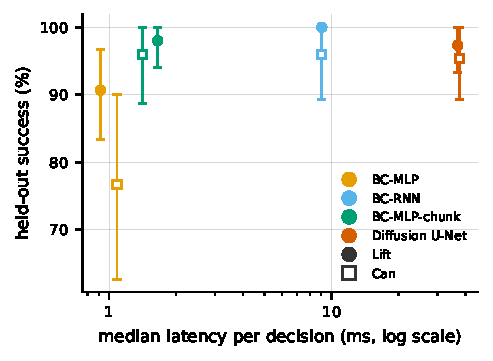
\includegraphics[width=0.8\linewidth]{generated/figures/latency_success.pdf}
\caption{Held-out success against the median latency of one decision (log scale) for the
Level~1 families, with the bootstrap interval. Filled circles: Lift; open squares: Can.}
\label{fig:latency}
\end{figure}
